% Discrete Continuous
\documentclass[tikz = true, border = 2pt]{standalone}

\usepackage{amsmath}
\usepackage{amsfonts}
\usepackage{amssymb}
\usepackage{graphicx}
\usepackage{tikz}
\usetikzlibrary{positioning, calc}
\usetikzlibrary{intersections}
\usetikzlibrary{decorations.pathreplacing}
\usetikzlibrary{decorations.text}
\usetikzlibrary{arrows,shapes,backgrounds, shadows,fadings}
\usepackage{fontspec}
\setmainfont{Equity Text A}[SmallCapsFont={Equity Caps A}, Numbers=Lining]
\begin{document}

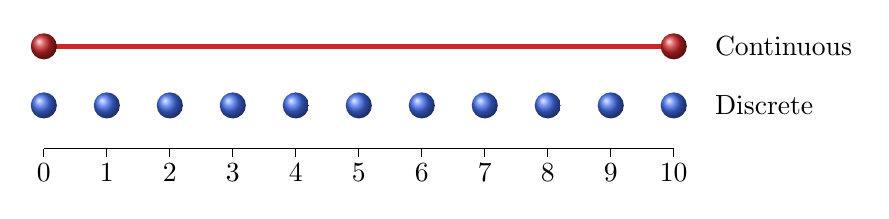
\begin{tikzpicture}[xscale=0.8]
\definecolor{firebrick2}{RGB}{205,38,38};
\definecolor{royalblue2}{RGB}{67,110,238};
\node [anchor=west] at (10.5,1) {Discrete};
\node [anchor=west] at (10.5,1.75) {Continuous};
\foreach \n in {0,...,10} {
	\node at (\n,0.15) {\n};
	\draw (\n,0.35)--(\n,0.45);
}
\tikzstyle{every node}=[draw=none,
                        shape=circle,
                        ball color=royalblue2,
                        minimum size=1mm];
\foreach \n in {0,...,10} {
	\node at (\n,1) {};
}
\draw (0,0.45) --(10,0.45);
\tikzstyle{every node}=[draw=none,
                        shape=circle,
                        ball color=firebrick2,
                        minimum size=1mm];
\draw [color=firebrick2,ultra thick] (0,1.75)--(10,1.75);                        
\node (r1) at (0,1.75) {};
\node  (r10)  at (10,1.75) {};

\end{tikzpicture}
\end{document}
